\section{函数的概念}
什么是函数?它是数学意义上的函数吗?\par
在数学意义上,一个函数$f$是从一个集合$\mathbb{X}$(值域)到另一个集合$\mathbb{Y}$(到达域)的某种映射关系\footnote{这里介绍数学意义上的函数,只为引入编程意义上的函数概念。如果读者拥有相关数学基础,自然更好;即便没有相关数学基础,也不妨碍对后续知识的理解和应用。}。对于$\mathbb{X}$集合中的某个元素$x$来说,总有唯一确定的$\mathbb{Y}$集合中的元素$y=f(x)$与之对应。举例来说,我们记$f(x)=x^2+2x+1$,其中$x\in\mathbb{R}$,那么对于某个输入$x=3$,就能通过这个函数算出$f(3)=16$来,这个结果就是函数的输出。\par
三角函数也是数学意义上的函数。比如正弦函数,它的名字就是$\sin$。不过它不像我们刚才用到的$f$那样,我们不知道它的表达式,如果你要问我$\sin1$是多少,我也不方便徒手计算,要用计算器才行。但是无论何时何地,我算出的$\sin1$和张三算出的$\sin1$、李四算出的$\sin1$都是一样的。所以说,$\sin$的输入信息和输出信息之间有确定的对应关系。
我不知道$\sin$的内部构造,也不知道计算器是用什么原理来实现的,但是我给它某个输入,它就会给我对应的输出,这就是一个\textbf{黑盒(Black box)}(见图4.1)。\par
\begin{figure}[htbp]
    \centering
    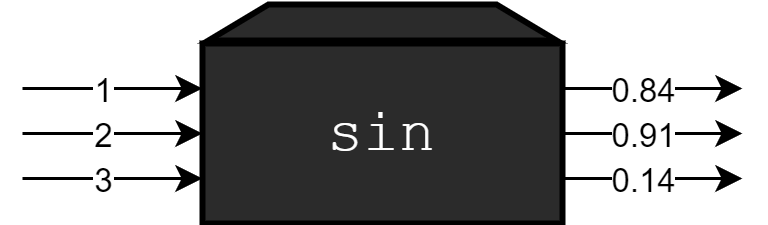
\includegraphics[width=0.4\textwidth]{../images/generalized_parts/04_black_box.drawio.png}
    \caption{$\sin$函数就是一个黑盒,给定某个输入信息就会有对应的输出信息}
\end{figure}
在编程当中,函数的概念可以借用数学上的函数概念来阐释。举个例子,\lstinline@cmath@ 库中有一个函数 \lstinline@sin@,它可以接收一个 \lstinline@double@ 类型的参数,并返回一个 \lstinline@double@ 类型的结果。所以我们可以说它的定义域$\mathbb{X}$就是 \lstinline@double@ 型的所有数据,到达域$\mathbb{Y}$也是 \lstinline@double@ 型的所有数据。\par
\begin{lstlisting}
#include <iostream> //标准输入输出头文件
#include <cmath> //sin函数定义在cmath库中
using namespace std; //使用命名空间std
int main() {
    cout << sin (3.14159); //使用sin函数求出sin(3.14159)的值
    return 0;
}
\end{lstlisting}
这段代码的输出是\\\noindent\rule{\textwidth}{0.2pt}\texttt{
2.65359e-06
}\\\noindent\rule{\textwidth}{0.2pt}\\
它是一个非常小的数,这是合乎我们的预期的。\footnote{注意,\lstinline@cmath@ 库中的 \lstinline@sin@ 函数接收的参数是按照弧度值传入的,所以$\sin3.14159\approx0$。}\par
数学上还有多元函数的概念,也就是接收一个或多个输入,并给出一个输出的函数。在程序设计中,函数也可以接收一个或多个输入,甚至接收空输入(我们在前面用到的 \lstinline@numeric_limits<int>::max()@ 就是一个空输入的函数)。但是函数只能返回一个输出\footnote{如果我们需要让返回多个值,可以使用结构体 \lstinline@struct@ 或者 \lstinline@std::tuple@。我们将来会接触到这种情况的。但这并不违反``至多只能返回一个输出''的规定,因为一整个结构体或 \lstinline@tuple@ 就是单个输出。}或者返回 \lstinline@void@\footnote{\lstinline@void@ 也是一个基本数据类型,但它不能用来定义数据,可以用来定义指针。在函数中,我们会经常见到这种类型的。}(即空输出)。我们在下一节中就会提到这些。\par
我们熟识的运算符就可以看成是一种函数\footnote{实际上运算符和函数并不相同,不过它们有很多相似之处,可以用于类比。}。加法运算符就是一个黑盒,它的两个操作数就是两个输入信息,而返回值(输出信号)就是它们的和。运算符中有操作数和返回值的概念,这些概念对应到函数中就是参数和返回值。\par
C++的各种库为我们提供了许多函数,我们可以直接使用这些函数来实现我们想要的功能,而不需要自己把每个功能实现出来。比如说 \lstinline@cmath@ 库中有丰富的数学函数,除了刚才的正弦函数以外,还有求绝对值函数 \lstinline@abs@、开平方函数 \lstinline@sqrt@、下取整函数 \lstinline@floor@ 等。如果真的要我们自己写代码实现的话,这是非常麻烦的(试想,如何用一些结构控制语句和四则运算来求开平方呢?这好像很难办到)。\par
而C++的函数封装了一些已经实现好的功能,我们不再需要考虑如何写一个开方代码,思路是什么,需要注意哪些细节——直接用 \lstinline@cmath@ 库给我们的解决方案就好了。
\begin{lstlisting}
    double num; //定义一个num用来接收输入
    cin >> num; //输入num的值
    cout << sqrt (num); //输出num开方后的值
\end{lstlisting}\par
我们还可以自己定义函数。比如在\hyperref[lst:SumWithContinue]{代码3.4}中,我提供了一个 \lstinline@input_clear@ 函数,用来请除 \lstinline@cin@ 的错误状态并清理本行输入。这个函数在其它地方也可以用\footnote{前提是需要定义,或者声明并在有关的代码中提供了定义。详见下一节。},只需要写一个 \lstinline@input_clear();@ 就可以了,而不需要把函数体当中的那三行代码再写一遍——这样就很方便了。\par
而且更重要的是,如果我有朝一日不使用 \lstinline@cin@ 而是用别的来进行输入(还记得吗?\lstinline@cin@ 只是 \lstinline@istream@ 类的一个对象,我们还可以使用这个类或者派生类\footnote{有关继承和派生类的概念,我们将在第九章介绍。}的其它对象来进行输入),那么我只需要在 \lstinline@input_clear@ 的定义中修改一次即可。但如果我不用函数而是每次都写那三行代码呢?修改起来也会相当麻烦。\par
使用函数还有一个优点,我们可以把一个复杂的大任务拆分成几个简单的小任务。其实在之前写代码的过程中,我们也是有意把程序的思路梳理清楚的,这个功能应该怎么做,那个功能应该怎么做。而函数看上去更加直观,我们为每一项操作起了一个名字,然后分别把它们写到不同的代码中去,这样就方便很多了。\par
接下来我们就开始学习如何定义和使用函数,以后我们会频繁用到的。鉴于我们还有很多复合数据类型相关的知识没有学习,本章只是对函数作一些初步讲解。\par
